\section{Conclusions and future work}
\label{sec:concl}
In this work, we have expanded our data base of 356 optimally bipartitioned sparse matrices
to 839 matrices, by developing a new flow-based bound for our previous branch-and-bound algorithm~\cite{pelt15}.
We implemented this bound in a new matrix partitioner, MP, which has the same functionality as the 
previous partitioner MondriaanOpt.
We are now able to bipartition 96.8\% of the sparse matrices with at most 1000 nonzeros
from the SuiteSparse collection~\cite{davis11}
to optimality, reaching the exact minimum communication volume for a given load imbalance $\epsilon=0.03$. 
For matrices with less than 10,000 nonzeros, we are successful in 72.8\% of the cases,
and for matrices with less than 100,000 nonzeros still in 52.3\%.    
The new partitioner MP is 11.7 times faster than MondriaanOpt for problems that both
partitioners can solve, but more importantly it enables us to solve many more partitioning problems.

In the near future, we intend to apply the new partitioner also to selected  problems that we could not solve
within our imposed limit of 24 hours. Looking already beyond the horizon,
we bipartitioned the matrix \texttt{cage6} using MP in 283,316 s (over 3 days) on a laptop computer.
Extrapolating the timing behaviour of our previous solver MondriaanOpt,
we estimate that this would have taken 2 years of CPU time for that solver.
The matrix \texttt{cage6} is the smallest matrix (in terms of number of nonzeros) that could not be solved within 24 hours
by MP.
The result of the 3-day calculation is shown in Fig.~\ref{fig:cage6}.

In this paper, we also gave a proof of the NP-completeness of the balanced sparse matrix bipartitioning problem,
where both parts obtain an equal number of nonzeros. This result may hardly be surprising,
as graph partitioning and hypergraph partitioning are both known to be NP-complete.
Still, this problem is a very specific instance of hypergraph partitioning,
and it is a motivation for developing good heuristic partitioners to know that solving the problem optimally
by an exact algorithm is intractable.
It is our hope that the expanded data base of optimally bipartitioned sparse matrices
will be used in practice to benchmark the quality of
the bipartitioning kernel of such heuristic partitioners.

\begin{figure}[htbp]
\label{fig:cage6}
  \centering
  \frame{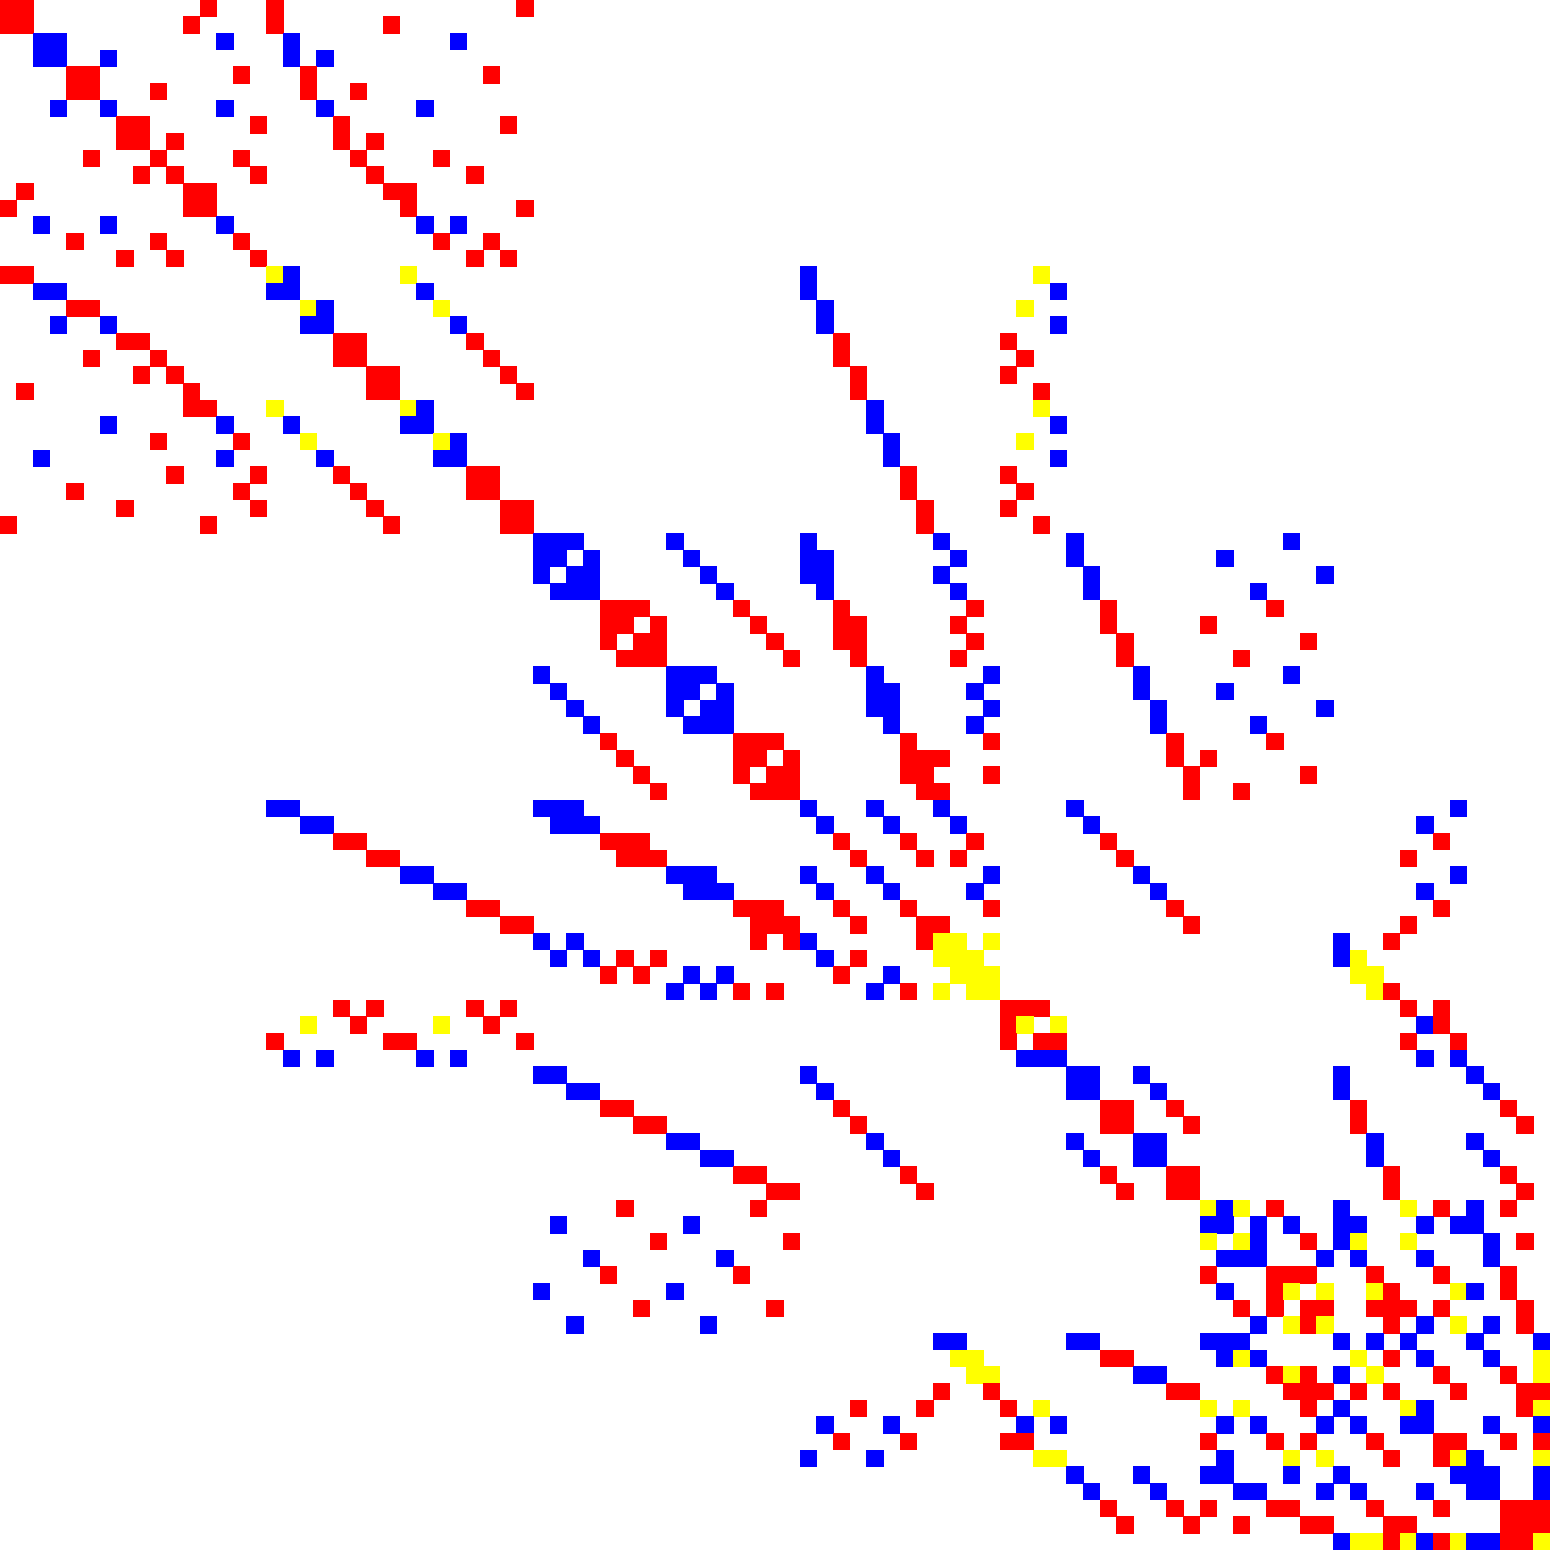
\includegraphics[width=8cm]{cage6.pdf}}
  \caption{Bipartitioning of the $93 \times 93 $ matrix \texttt{cage6} with 785 nonzeros.
The minimum communication volume for an allowed imbalance of $\epsilon=0.03$ equals $V=38$. 
The 397 red nonzeros are assigned to one part, the 316 blue nonzeros to the other part,
and the 72 yellow nonzeros can be freely assigned to any part without affecting
the communication volume, because both their row and their column is already cut.
We can color these free nonzeros to improve the load balance, giving 397 red and 388 blue nonzeros,
corresponding to an achieved imbalance of about $\epsilon^{\prime}=0.01$.}
\end{figure} 
